\documentclass[portrait,final,a0paper]{baposter}


\tracingstats=2

\usepackage{calc}
\usepackage{graphicx}
\usepackage{amsmath}
\usepackage{amssymb}
\usepackage{relsize}
\usepackage{multirow}
\usepackage{bm}

\usepackage{graphicx}
\usepackage{multicol}

\usepackage{pgfbaselayers}
\pgfdeclarelayer{background}
\pgfdeclarelayer{foreground}
\pgfsetlayers{background,main,foreground}

\usepackage{times}
\usepackage{helvet}
%\usepackage{bookman}
\usepackage{palatino}

\newcommand{\captionfont}{\footnotesize}

\selectcolormodel{cmyk}

%\graphicspath{{images/}}

%%%%%%%%%%%%%%%%%%%%%%%%%%%%%%%%%%%%%%%%%%%%%%%%%%%%%%%%%%%%%%%%%%%%%%%%%%%%%%%%
%%%% Some math symbols used in the text
%%%%%%%%%%%%%%%%%%%%%%%%%%%%%%%%%%%%%%%%%%%%%%%%%%%%%%%%%%%%%%%%%%%%%%%%%%%%%%%%
% Format 

\renewcommand{\Pr}{\mbox{P}}
\newcommand{\e}{\mbox{e}}
%%%%%%%%%%%%%%%%%%%%%%%%%%%%%%%%%%%%%%%%%%%%%%%%%%%%%%%%%%%%%%%%%%%%%%%%%%%%%%%%
% Multicol Settings
%%%%%%%%%%%%%%%%%%%%%%%%%%%%%%%%%%%%%%%%%%%%%%%%%%%%%%%%%%%%%%%%%%%%%%%%%%%%%%%%
\setlength{\columnsep}{0.7em}
\setlength{\columnseprule}{0mm}


%%%%%%%%%%%%%%%%%%%%%%%%%%%%%%%%%%%%%%%%%%%%%%%%%%%%%%%%%%%%%%%%%%%%%%%%%%%%%%%%
% Save space in lists. Use this after the opening of the list
%%%%%%%%%%%%%%%%%%%%%%%%%%%%%%%%%%%%%%%%%%%%%%%%%%%%%%%%%%%%%%%%%%%%%%%%%%%%%%%%
\newcommand{\compresslist}{%
\setlength{\itemsep}{1pt}%
\setlength{\parskip}{0pt}%
\setlength{\parsep}{0pt}%
}


%%%%%%%%%%%%%%%%%%%%%%%%%%%%%%%%%%%%%%%%%%%%%%%%%%%%%%%%%%%%%%%%%%%%%%%%%%%%%%
%%% Begin of Document
%%%%%%%%%%%%%%%%%%%%%%%%%%%%%%%%%%%%%%%%%%%%%%%%%%%%%%%%%%%%%%%%%%%%%%%%%%%%%%

\begin{document}

%%%%%%%%%%%%%%%%%%%%%%%%%%%%%%%%%%%%%%%%%%%%%%%%%%%%%%%%%%%%%%%%%%%%%%%%%%%%%%
%%% Here starts the poster
%%%---------------------------------------------------------------------------
%%% Format it to your taste with the options
%%%%%%%%%%%%%%%%%%%%%%%%%%%%%%%%%%%%%%%%%%%%%%%%%%%%%%%%%%%%%%%%%%%%%%%%%%%%%%
% Define some colors
\definecolor{silver}{cmyk}{0,0,0,0.3}
\definecolor{yellow}{cmyk}{0,0,0.9,0.0}
\definecolor{reddishyellow}{cmyk}{0,0.22,1.0,0.0}
\definecolor{black}{cmyk}{0,0,0.0,1.0}
\definecolor{darkYellow}{cmyk}{0,0,1.0,0.5}
\definecolor{darkSilver}{cmyk}{0,0,0,0.1}

\definecolor{lightyellow}{cmyk}{0,0,0.3,0.0}
\definecolor{lighteryellow}{cmyk}{0,0,0.1,0.0}
\definecolor{lighteryellow}{cmyk}{0,0,0.1,0.0}
\definecolor{lightestyellow}{cmyk}{0,0,0.05,0.0}
\definecolor{cyan}{cmyk}{1,0,0,0}
\definecolor{lightcyan}{cmyk}{0.5,0,0,0}
\definecolor{pastelcyan}{cmyk}{0.25,0,0,0}
\definecolor{magenta}{cmyk}{0,1,0,0}
\definecolor{yellow}{cmyk}{0,0,1,0}
\definecolor{lightyellow}{cmyk}{0,0,0.5,0}
\definecolor{pastelyellow}{cmyk}{0,0,0.25,0}
\definecolor{black}{cmyk}{0,0,0,1}
\definecolor{darkgray}{cmyk}{0,0,0,0.75}
\definecolor{gray}{cmyk}{0,0,0,0.5}
\definecolor{lightgray}{cmyk}{0,0,0,0.25}
\definecolor{white}{cmyk}{0,0,0,0}
\definecolor{red}{cmyk}{0,1,1,0}
\definecolor{orange}{cmyk}{0,0.5,1,0}
\definecolor{scarlet}{cmyk}{0,1,0.5,0}
\definecolor{brown}{cmyk}{0.5,0.75,1,0}
\definecolor{camel}{cmyk}{0.25,0.375,0.5,0}
\definecolor{cream}{cmyk}{0,0.2,0.3,0}
\definecolor{green}{cmyk}{1,0,1,0}
\definecolor{lightgreen}{cmyk}{0.5,0,0.5,0}
\definecolor{pastelgreen}{cmyk}{0.25,0,0.25,0}
\definecolor{mossgreen}{cmyk}{0.64,0.4,1,0}
\definecolor{yellowgreen}{cmyk}{0.5,0,1,0}
\definecolor{skyblue}{cmyk}{0.4,0.16,0,0}
\definecolor{royal}{cmyk}{1.0,0.5,0,0}
\definecolor{navyblue}{cmyk}{0.9,0.75,0.5,0}
\definecolor{lightnavy}{cmyk}{0.4,0.3,0.2,0}
\definecolor{blue}{cmyk}{1,1,0,0}
\definecolor{lightblue}{cmyk}{0.5,0.5,0,0}
\definecolor{pastelblue}{cmyk}{0.25,0.25,0,0}
\definecolor{lightpastelblue}{cmyk}{0.15,0.15,0,0}
\definecolor{lightestpastelblue}{cmyk}{0.05,0.05,0,0}
\definecolor{lavender}{cmyk}{0.25,0.25,0,0}
\definecolor{violet}{cmyk}{0.75,1,0.25,0}
\definecolor{purple}{cmyk}{0.5,1,0.5,0}
\definecolor{lightpurple}{cmyk}{0.25,0.5,0.25,0}
\definecolor{pink}{cmyk}{0,0.5,0,0}


%%
\typeout{Poster Starts}


\newlength{\leftimgwidth}
\begin{poster}%
  % Poster Options
  {
  % Show grid to help with alignment
  grid=false,
  % Column spacing
  colspacing=1em,
  % Color style
  %bgColorOne=lighteryellow,
  %bgColorTwo=lightestyellow,
  %borderColor=reddishyellow,
  %headerColorOne=yellow,
  %headerColorTwo=reddishyellow,
  %headerFontColor=black,
  %boxColorOne=lightyellow,
  %boxColorTwo=lighteryellow,
  bgColorOne=white,
  bgColorTwo=white,
  borderColor=navyblue,
  headerColorOne=lightnavy,
  headerColorTwo=purple,
  headerFontColor=black,
  boxColorOne=white,
  boxColorTwo=white,
  % Format of textbox
  %textborder=roundedleft,
  textborder=rectangle,
  % Format of text header
  eyecatcher=true,
  headerborder=open,
  headerheight=0.08\textheight,
 % headershape=roundedright,
  headershape=rectangle,
  headershade=plain,
  headerfont=\Large\textsf, %Sans Serif
  boxshade=plain,
%  background=shade-tb,
 % background=plain,
  background=none,
  linewidth=2pt
  }
  % Eye Catcher
  {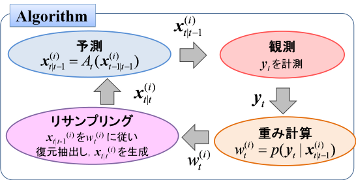
\includegraphics[width=13em]{pf}} % No eye catcher for this poster. (eyecatcher=no above). 
% If an eye catcher is present, the title is centered between eye-catcher and logo.
  % Title
  {\sf %Sans Serif
  %\bf% Serif
  Portfolio Optimisation\\with Sequential Monte Carlo}
  % Authors
  {\sf %Sans Serif
  % Serif
   Yow Tzu Lim (ytl13@imperial.ac.uk) \\ Supervisor: Dr. Nikolas Kantas
  }
  % University logo
  {% The makebox allows the title to flow into the logo, this is a hack because of the L shaped logo.
    \makebox[8em][r]{%
      \begin{minipage}{16em}
        \hfill
        
\includegraphics[height=4em]{imperial.pdf}
      \end{minipage}
    }
  }

  \tikzstyle{light shaded}=[top color=baposterBGtwo!30!white,bottom color=baposterBGone!30!white,shading=axis,shading angle=30]

  % Width of left inset image
     \setlength{\leftimgwidth}{0.78em+8.0em}

%%%%%%%%%%%%%%%%%%%%%%%%%%%%%%%%%%%%%%%%%
%%% Now define the boxes that make up the poster
%%%---------------------------------------------------------------------------
%%% Each box has a name and can be placed absolutely or relatively.
%%% The only inconvenience is that you can only specify a relative position 
%%% towards an already declared box. So if you have a box attached to the 
%%% bottom, one to the top and a third one which should be in between, you 
%%% have to specify the top and bottom boxes before you specify the middle 
%%% box.
%%%%%%%%%%%%%%%%%%%%%%%%%%%%%%%%%%%%%%%%%%
    %
    % A coloured circle useful as a bullet with an adjustably strong filling
    \newcommand{\colouredcircle}[1]{%
      \tikz{\useasboundingbox (-0.2em,-0.32em) rectangle(0.2em,0.32em); \draw[draw=black,fill=baposterBGone!80!black!#1!white,line width=0.03em] (0,0) circle(0.18em);}}

%%%%%%%%%%%%%%%%%%%%%%%%%%%%%%%%%%%%%%%%%%
\headerbox{About}{name=about,column=0,row=0}{
Portfolio optimisation is about efficiently allocating resources to achieve optimal investment objectives. Two usual objectives are maximising return and minimizing the returns. \\

This project views portfolio optimisation problem as a finite horizon control optimisation problem, and uses sequential monte carto (SMC) to search for the optimised control (investment decision).
	\vspace{0.5em}
 }

%%%%%%%%%%%%%%%%%%%%%%%%%%%%%%%%%%%%%%%%
  \headerbox{Porfolio Optimisation}{name=po,column=0,below=about}{
  
We begin to view the market consisting of $N$ investible instruments. The price of an instrument $S_i$ is assumed to follow an arithmetic Brownian motion as follows:
\begin{equation}
  dS(t) = \mu dt + \sigma dW(t)
\end{equation}
with initial condition $S_0 > 0$, $\mu$ is the average rate of return and $\sigma$ is the volatility (risk).
\\

Let $u(t)$ denote the number of shares of the asset one holds, then the value of the corresponding asset is a process $X(t)$ that evolves according to
\begin{equation}
  dX(t) = \mu u(t) dt + \sigma u(t) dW(t)
\end{equation}

The objective is to maximize the expected return over a fixed time interval $[0,T]$, at the same time minimizing the financial risk.

  \vspace{0.5em}
  }

%%%%%%%%%%%%%%%%%%%%%%%%%%%%%%%%%%%%%%%
\headerbox{Stochastic Control}{name=sc,column=0,below=po}{
In control theory, performance is often expressed in terms of total reward (or total cost), $J_x$, which is an expectation of some function.
\\

Decision maker cannot see the future, current decisions affect only future states and observations. Some possible settings include:
\begin{enumerate}
\item  Total cost function (additive vs.\ multiplicative)
\begin{equation}
J^a_X = E_X[\sum^T_{n=1} j^a_i(X_n, U_n, Y_n)] \\
\end{equation}
\begin{equation}
J^a_X = E_X[\prod^T_{n=1} j^a_n(X_n, U_n, Y_n)]
\end{equation}
where $j^a_n$ is stage cost at time $n$.
\item Finite/infinite horizon T.
\item Open loop vs.\ closed loop (feedback).
\item Perfect vs. imperfect observation.
\end{enumerate}
%  \vspace{0.5em}
  }

%%%%%%%%%%%%%%%%%%%%%%%%%%%%%%%%%%%%%%%
\headerbox{Open loop control as Bayesian filtering}{name=bf,column=1,span=2, row=0}{
An example of non-linear time-varying dynamic system:
\begin{align*}
 X_n &= F_n(X_{n-1}, U_n)\\
 Y_n &= h_n(X_n)
\end{align*}
where $X_n$ are the markov chain state spaces, $Y_n$ are the observations and $U_n$ are the controls. \\

Let $A_n$ and $B_n$ be symmetric and semi-definite positive covariance matrices, a simple possible {\bf finite horizon cost function} as follows:
\begin{equation}
  J(U_{1:T}, Y_{1:T}) = \sum^T_{n=1} \|U_n\|^2_{A_n} + \sum^T_{n=1} \|Y_n - Y^{ref}\|^2_{B_n}
\end{equation}
where $Y^{ref}$ represent the reference target output, and $\|U\|^2_{A} = U^TA^{-1}U$.
\\

{\bf Objective:} Search for an optimal policy (sequence of investment decisions) that minimize the cost control function, given some observations.
\vspace{0.5em}
}

%%%%%%%%%%%%%%%%%%%%%%%%%%%%%%%%%%%%%%%
\headerbox{Sequntial Monte Carlo (SMC)}{name=smc,column=1,span=2, below=bf}{
%%%%%%%%%%%%%%%%%%%%%%%%%%%%%%%%%%%%%%%
A swarm of particles (samples), that evolves towards the target distribution throughout sequence of intermediate distributions $\{\pi_n\}_{n \leq T}$.\\

The particles that approximates the intermediate distributions $\pi_n$ are construsted based on the particles from $\pi_{n-1}$ via sampling and re-sampling.\\

\begin{center} 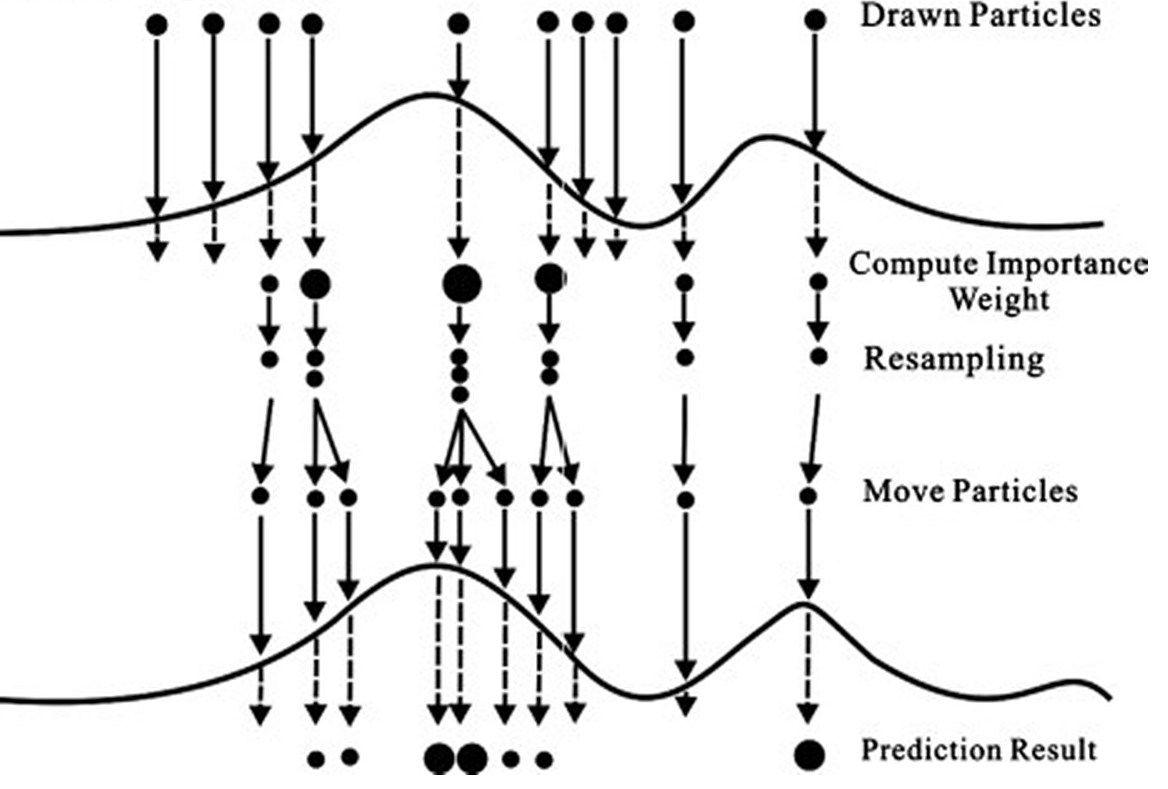
\includegraphics[height=5cm]{smc.png} \end{center}

{\bf Optional step: } MCMC step can be adeed to each iteration to improve diversity of the particles.
  \vspace{0.5em}
  }

%%%%%%%%%%%%%%%%%%%%%%%%%%%%%%%%%%%%%%%%	
\headerbox{SMC Algorithm for estimating open loop controls}{name=algo,column=1,span=2,below=smc}{
For each time step $n \in  {1 \dots T}$, 
  \begin{enumerate}
        \item For $i \in {1 \dots N}$, where $N$ is number of particles, 
            \begin{enumerate}
	        \item If $n == 1$, initialize $x^i = x_0$, $y^i= h(x_0)$ and $J^i_T = 0$.
    	        \item Generate random $u^i \sim N(0, A_n)$.
    	        \item Store action to a list $u^i_n = u ^ i$.
            \item Evaluate $J_y = \|y^{ref}_n\|^2_{B_n}$, $J^i_T = \|u^i\|^2_{A_n}$ and calculate the cost $J^i_T = J^i_T + J^i_Y + J^i_U$
            \item Set weight $p^i_{un} = \exp(-\dfrac{\beta}{2} J_Y)$.
            \end{enumerate}
        \item Normalize resampling probabilities: For $i \in {1 \dots N}$, $p^i = \dfrac{p^i_{un}}{\sum^N_{i=1}p^i_{un}}$
        \item Resample:  For $i \in {1 \dots N}$, select particles with replacement according to $p^i$.
        \item Compute model for next time step $n$: $x^i = f(x^i, u^i)$ and $y^i = h(x^i)$.
  \end{enumerate}
Find $i^* = \arg\min_i J^i_T$. The solution for the optimal control is $v^{i^*}$.

  \vspace{0.5em}
  }
%For all $i \in {1,\dots,N}$
%\begin{enumerate}
%\item Initialisation at time $t=1$ \\
%  \begin{enumerate}
%  	\item Sample $u^i_{1,1} \sim q(u_1)$
%  	\item Calculate $W^i_1 \propto \dfrac{G_1(u^i_{1,1})M_1(u_0,u^i_{1,1})}{q_1(u^i_{1,1})}, \sum^N_{i=1} W^i_1=1$
%  	\item Calculate $W^i_1 \propto G_1(u_{1,1})M_1(u)0,u^i_{1,1})$
%    \item Resample $\bar U^i_1 \sim \sum^N_{i=1} W^i_1 \delta_{u^i_{1,1}}(du_{1,1})$
%  \end{enumerate}
%\item Iteration at time $t$ in $2,3,\dots,T$ \\
%  \begin{enumerate}
%  	\item Sample $u^i_{1,1} \sim q(u_1)$
%  	\item Calculate $W^i_1 \propto \dfrac{G_1(u^i_{1,1})M_1(u_0,u^i_{1,1})}{q_1(u^i_{1,1})}, \sum^N_{i=1} W^i_1=1$
%  	\item Calculate $W^i_1 \propto G_1(u_{1,1})M_1(u)0,u^i_{1,1})$
%    \item Resample $\bar U^i_1 \sim \sum^N_{i=1} W^i_1 \delta_{u^i_{1,1}}(du_{1,1})$
%	\item Move
%  \end{enumerate}
%\item final step
%\end{enumerate} 	


\headerbox{Evaluation criteria}{name=eval,column=1,span=2,below=algo}{
Compare the performance against other optimisation algorithms, e.g., genetic algorithms:
\begin{enumerate}
\item Performance of the resulting policy
\item Computation complexity (many subroutines here can execute in parallel.)
\end{enumerate}
}

%\headerbox{Feedback?}{name=concl,column=1,span=2,above=bottom}{
%	\ \\
%	\ \\
%	\ \\
%	}
	
%%%%%%%%%%%%%%%%%%%%%%%%%%%%%%%%%%%%%%%
  \headerbox{References}{name=references,column=0,above=bottom}{
    \smaller
    \vspace{-0.4em}
    \bibliographystyle{plain}
    \renewcommand{\section}[2]{\vskip 0.05em}
      \begin{thebibliography}{1}\itemsep=-0.01em
      \setlength{\baselineskip}{0.4em}
      \bibitem{a}
        A. Doucet, S. Godsill, C. Andrieu
        \newblock On Sequential Monte Carlo Sampling Methods for Bayesian Filtering. 
        \newblock Statistics and Computing, vol. 10,  no. 3,  pp.197 -208, 2000
      \bibitem{n}
        N. Kantas, P. Del Moral, R. Vinter
        \newblock Particle methods for Stochastic Regulation: towards an application for power scheduling
        \newblock Technical Report, Imperial College, 2011
      \bibitem{m}
        M. Fischer and  G. Livieri
        \newblock Continuous time mean-variance portfolio optimization through the mean field approach.
        \newblock Pre-print, 2014      
      \bibitem{m}
	      E. Ikonen
        \newblock Particle Filtering for Open-Loop Process Control
        \newblock 2006      
      \end{thebibliography}
  }
%%%%%%%%%%%%%%%%%%%%%%%%%%%%%%%%%%%%%%%%%
  
\end{poster}

\end{document}
